\documentclass[12pt,a4paper]{article}

\usepackage[a4paper, top=2.5cm, bottom=2.5cm, left=2.5cm, right=2.5cm]{geometry}
\usepackage{iftex}

\ifPDFTeX
    \usepackage[utf8]{inputenc}
    \usepackage[T1]{fontenc}
    \usepackage[polish]{babel}
\else
    \usepackage{fontspec}
    \usepackage[polish, bidi=basic, provide=*]{babel}
    \babelprovide[import, onchar=ids fonts]{polish}
    \babelprovide[import, onchar=ids fonts]{english}
    \babelfont{rm}{Noto Sans}
\fi

\usepackage{enumitem}
\setlist[itemize]{label=-}

\usepackage{amsmath}
\usepackage{float}
\usepackage{graphicx}

\begin{document}

\section{Zestawienie danych początkowych}

Do obliczeń przyjęliśmy następujące parametry początkowe i geometryczne, są nieco inne niż te na tablicy ustalone w przypadku temperatury otoczenia i temperatury ścianki pieca:
\begin{itemize}
    \item Emisyjność materiału nagrzewanego (Inconel): $\epsilon_s = 0{,}50$
    \item Emisyjność wyłożenia izolacyjnego pieca: $\epsilon_k = 0{,}85$
    \item Stosunek powierzchni wsadu do komory: $\frac{S_s}{S_k} = \frac{0{,}0146}{0{,}4846} \approx 0{,}0301$
    \item Temperatura ścianki pieca: $T_k = 723{,}15\text{ K}$ ($450^\circ\text{C}$)
    \item Temperatura w punkcie $T_3$ ($R=0\text{ mm}$, $Z=130\text{ mm}$): $T_s = 479{,}20\text{ K}$ ($206{,}05^\circ\text{C}$)
    \item Temperatura otoczenia: $T_a = 21{,}85^\circ\text{C}$
\end{itemize}

\section{Obliczenia całkowitego współczynnika wymiany ciepła}

Całkowita gęstość strumienia ciepła $q_{\text{całk}}$ składa się z części radiacyjnej $q_{\text{rad}}$ oraz konwekcyjnej $q_{\text{kon}}$:
\begin{equation}
    q_{\text{całk}} = q_{\text{rad}} + q_{\text{kon}}
\end{equation}

\subsection{Promieniowanie ($q_{\text{rad}}$)}
\begin{equation}
    q_{\text{rad}} = \frac{5{,}67 \cdot 10^{-8} \cdot \left( T_k^4 - T_s^4 \right)}{\frac{1}{\epsilon_s} + \frac{S_s}{S_k} \left( \frac{1}{\epsilon_k} - 1 \right)}
\end{equation}

Podstawiając wartości pomiarowe dla termometru $T_3$:
\begin{equation}
    q_{\text{rad}} = \frac{5{,}67 \cdot 10^{-8} \cdot \left( 723{,}15^4 - 479{,}20^4 \right)}{\frac{1}{0{,}50} + 0{,}0301 \cdot \left( \frac{1}{0{,}85} - 1 \right)} = \frac{12509{,}67}{2{,}0053} \approx 6241{,}42 \text{ W/m}^2
\end{equation}

\subsection{Konwekcja ($q_{\text{kon}}$)}
Wartość wyznaczona z części konwekcyjnej:
\begin{equation}
    q_{\text{kon}} = 1686{,}65 \text{ W/m}^2
\end{equation}

\subsection{Całkowity strumień ciepła ($q_3$) i współczynnik $\alpha_3$}
\begin{equation}
    q_3 = q_{\text{rad}} + q_{\text{kon}} = 6241{,}42 + 1686{,}65 = 7928{,}07 \text{ W/m}^2
\end{equation}

Współczynnik wymiany ciepła dla różnicy temperatur $\Delta T = T_k - T_s = 243{,}95\text{ K}$:
\begin{equation}
    \alpha_3 = \frac{q_3}{T_k - T_s} = \frac{7928{,}07}{243{,}95} \approx 32{,}50 \text{ W/(m}^2\cdot\text{K)}
\end{equation}

\section{Analiza wyników i wykresy}

\subsection{Porównanie temperatury zmierzonej z obliczoną dla $\alpha_3 = 32{,}50 \text{ W/(m}^2 \cdot \text{K)}$}

Na rysunku \ref{fig:wykres_t3} przedstawiamy przebieg temperatury w funkcji czasu $T(\tau)$ uzyskany z symulacji numerycznej w programie \texttt{walec.exe} dla wyznaczonej przez nas wartości współczynnika wymiany ciepła $\alpha_3 = 32{,}50 \text{ W/(m}^2 \cdot \text{K)}$. Rysunek \ref{fig:porownanie_t1} zestawia nasze przebigi obliczeniowe dla trzech punktów pomiarowych ($T_1$, $T_2$, $T_3$).

\begin{figure}[H]
    \centering
    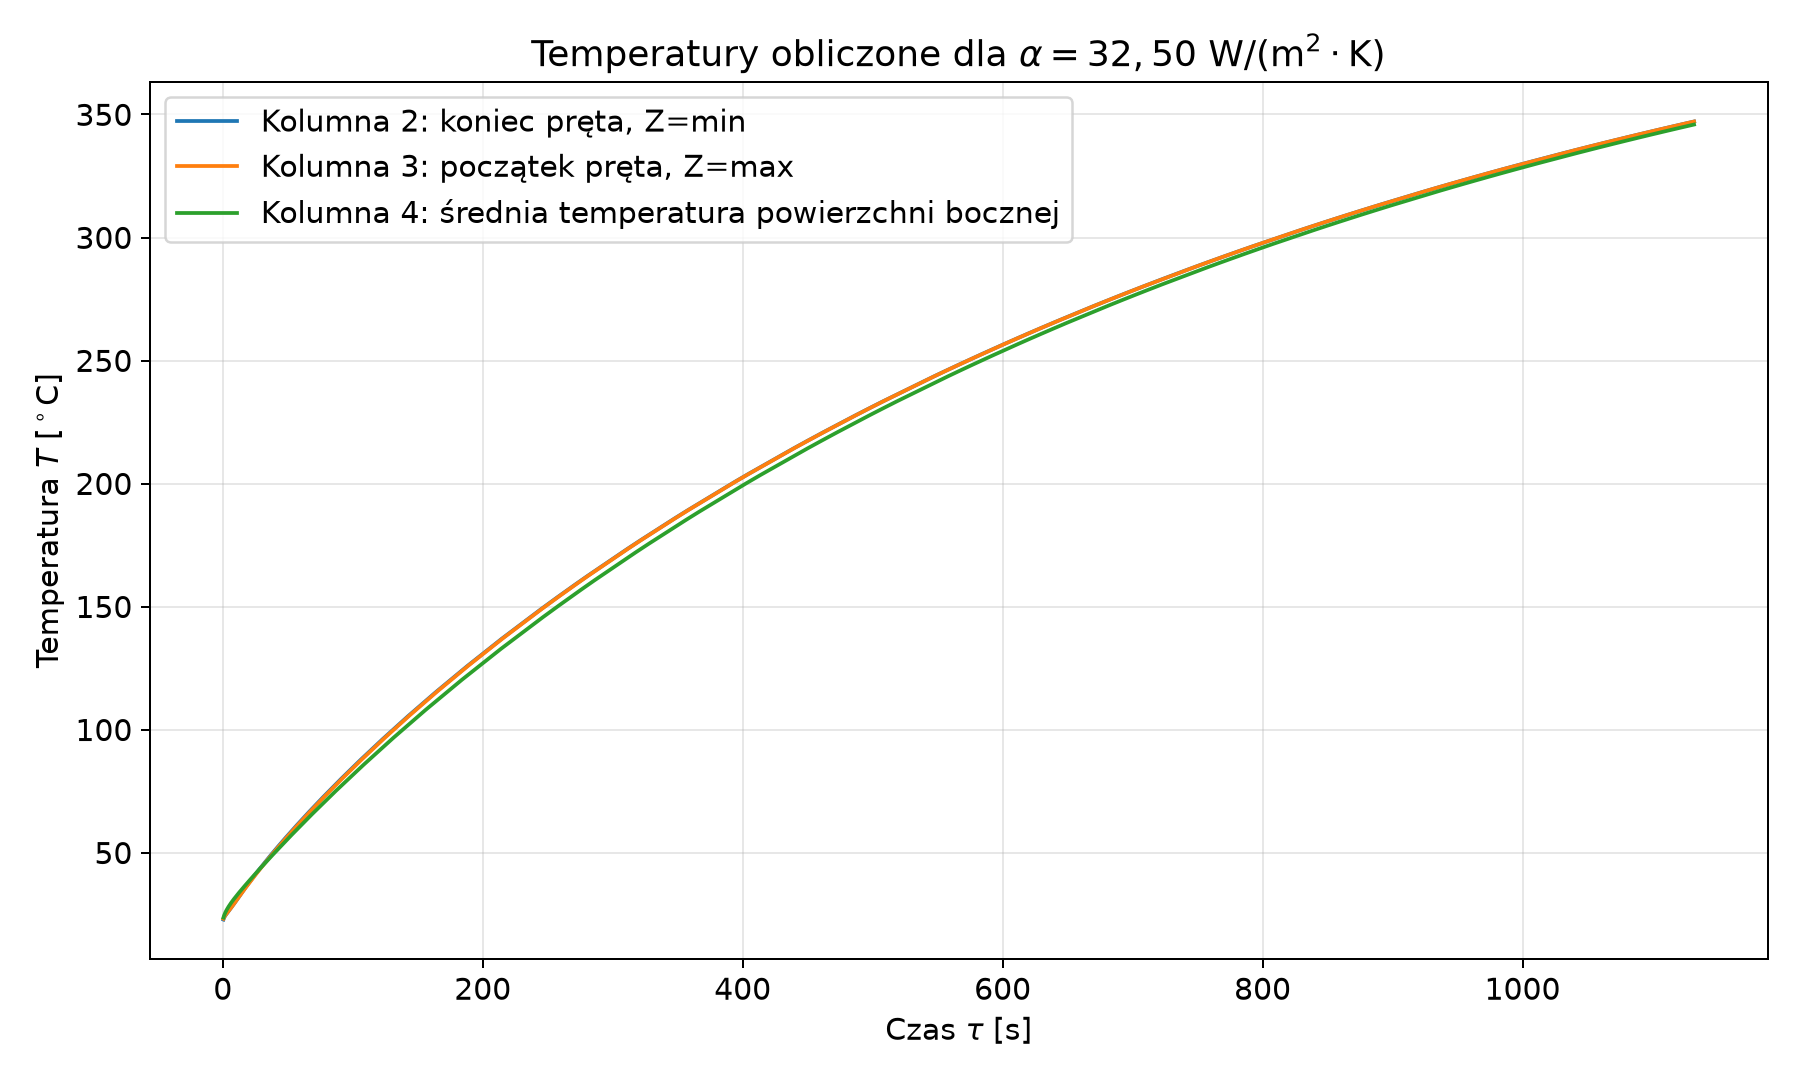
\includegraphics[width=0.92\textwidth]{temperatura_3_punkty.png}
    \caption{Wykres temperatury $T(\tau)$ w 3 punktach pomiarowych dla wyznaczonego analitycznie $\alpha_3 = 32{,}50 \text{ W/(m}^2 \cdot \text{K)}$.}
    \label{fig:wykres_t3}
\end{figure}

\begin{figure}[H]
    \centering
    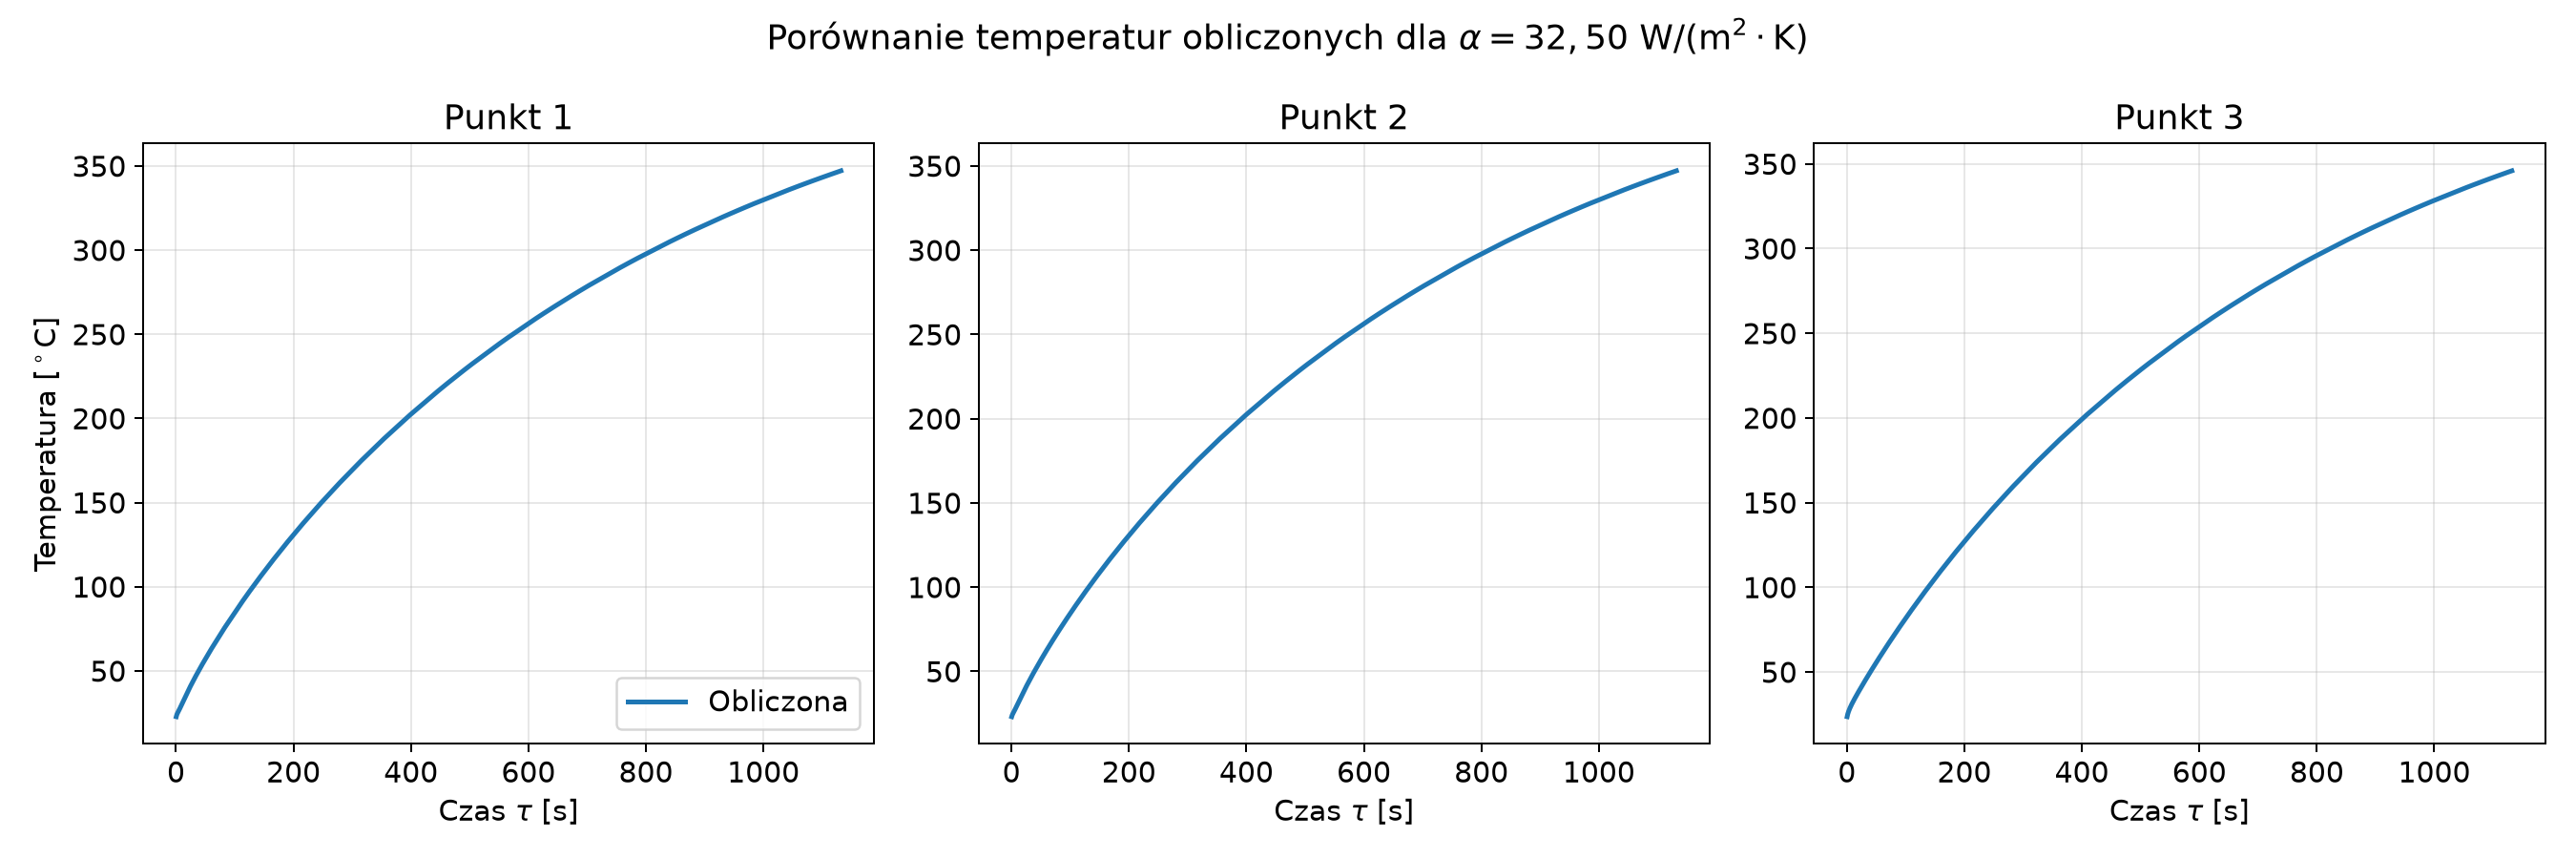
\includegraphics[width=\textwidth]{porownanie_T123.png}
    \caption{Porównanie przebiegów temperatur obliczonych dla trzech punktów pomiarowych przy $\alpha = 32{,}50 \text{ W/(m}^2 \cdot \text{K)}$.}
    \label{fig:porownanie_t1}
\end{figure}

Brak udostępnionej w formie szeregu czasowego tabeli \texttt{tpomiar.dat} z temperaturami zmierzonymi uniemożliwia nam bezpośrednie naniesienie krzywych pomiarowych na ten wykres. Dostępny plik \texttt{wcim wyniki 1.xlsx} zawiera wyłącznie zestawienie temperatur skrajnych i parametrów obliczeniowych, dlatego rys. \ref{fig:porownanie_t1} przedstawia nasze wyniki obliczeniowe we wszystkich trzech punktach, a pełne porównanie pomiar--obliczenie będzie możliwe po dołączeniu pełnego szeregu pomiarowego.

Do zestawienia zastosowano dane z pliku \texttt{wynik.txt} oraz \texttt{wynik wcim.xlsx}. Czas nagrzewania wynosi od $0{,}5$ do $1132{,}0$ s, a średnia temperatura powierzchni bocznej rośnie od $23{,}62$ do $345{,}92^\circ\text{C}$.

\subsection{Analiza gęstości strumienia ciepła $q_{\text{inv}}$ z zagadnienia odwrotnego}

W celu pełnej charakterystyki wymiany ciepła na powierzchni wsadu wyznaczyliśmy zależność gęstości strumienia ciepła $q_{\text{inv}}$ z rozwiązania zagadnienia odwrotnego. Na rysunku \ref{fig:qinv_Ts} przedstawiamy zmianę gęstości strumienia ciepła $q_{\text{inv}}$ w funkcji temperatury powierzchni $T_s$ (oś odciętych stanowi temperatura powierzchni $T_s$, oś rzędnych --- gęstość strumienia ciepła $q_{\text{inv}}$). Na rysunku \ref{fig:qinv_czas} przedstawiamy natomiast przebieg zmian gęstości strumienia ciepła $q_{\text{inv}}(\tau)$ w funkcji czasu nagrzewania.

\begin{figure}[H]
    \centering
    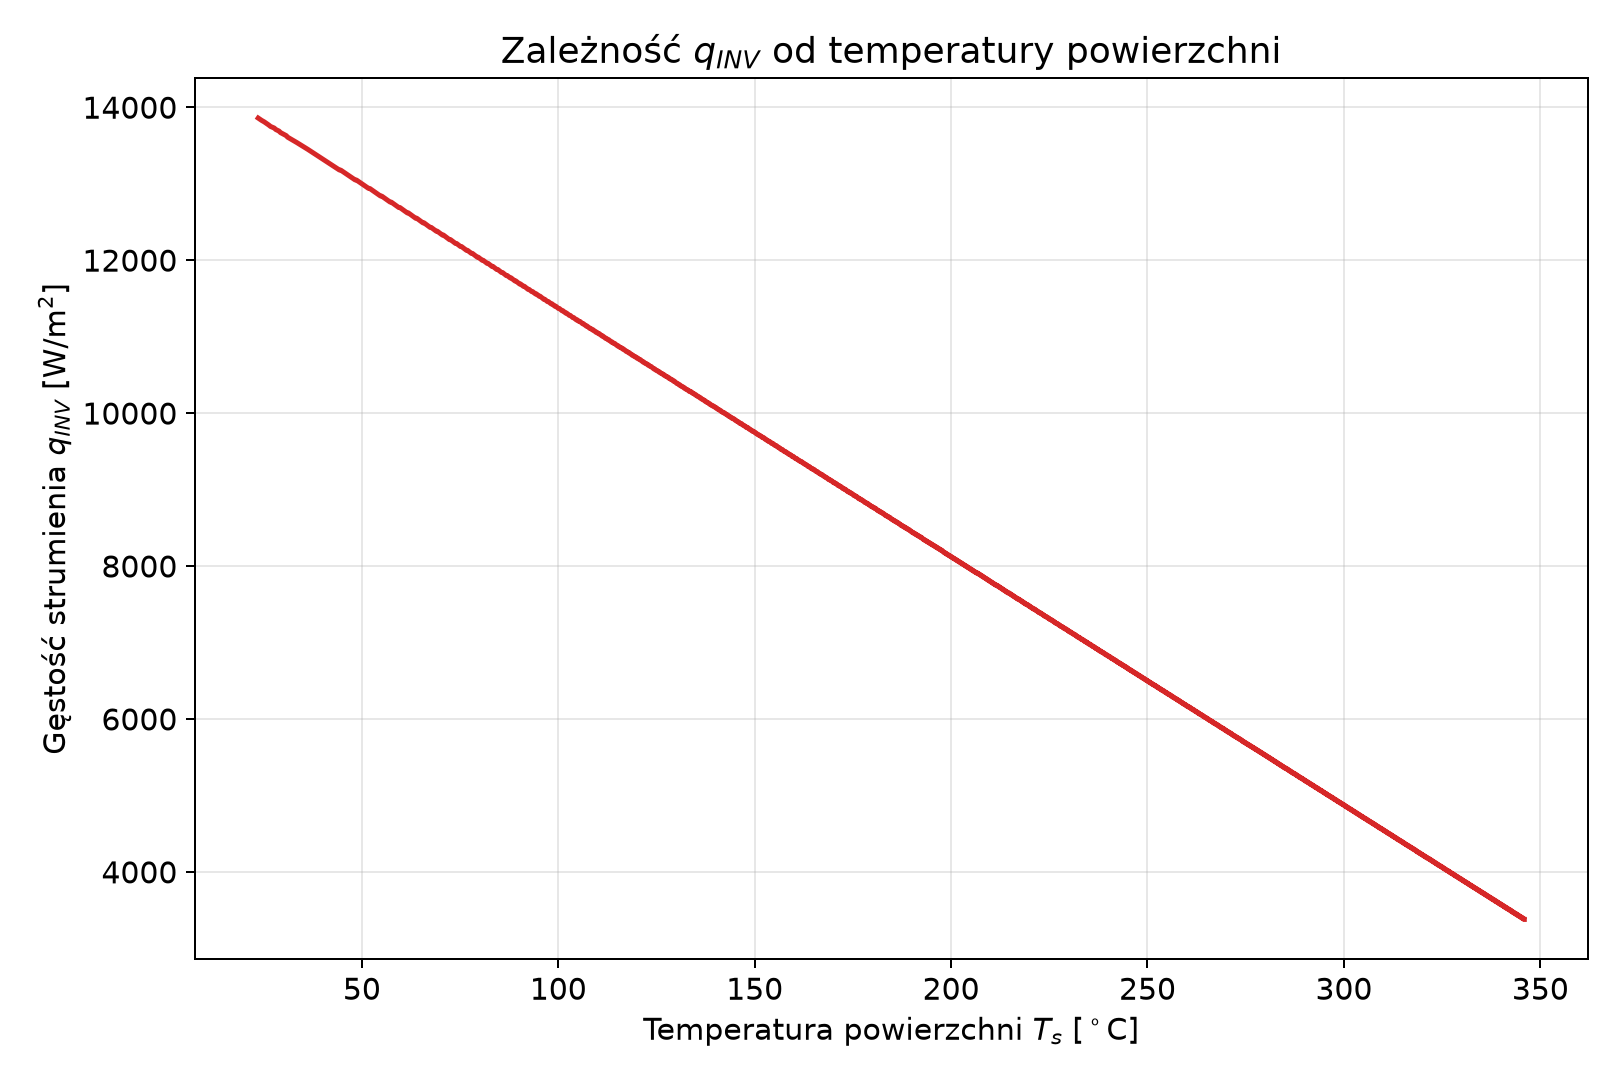
\includegraphics[width=0.92\textwidth]{wykres_qinv_Ts.png}
    \caption{Zmiana gęstości strumienia ciepła $q_{\text{inv}}$ w zależności od temperatury powierzchni $T_s$.}
    \label{fig:qinv_Ts}
\end{figure}

\begin{figure}[H]
    \centering
    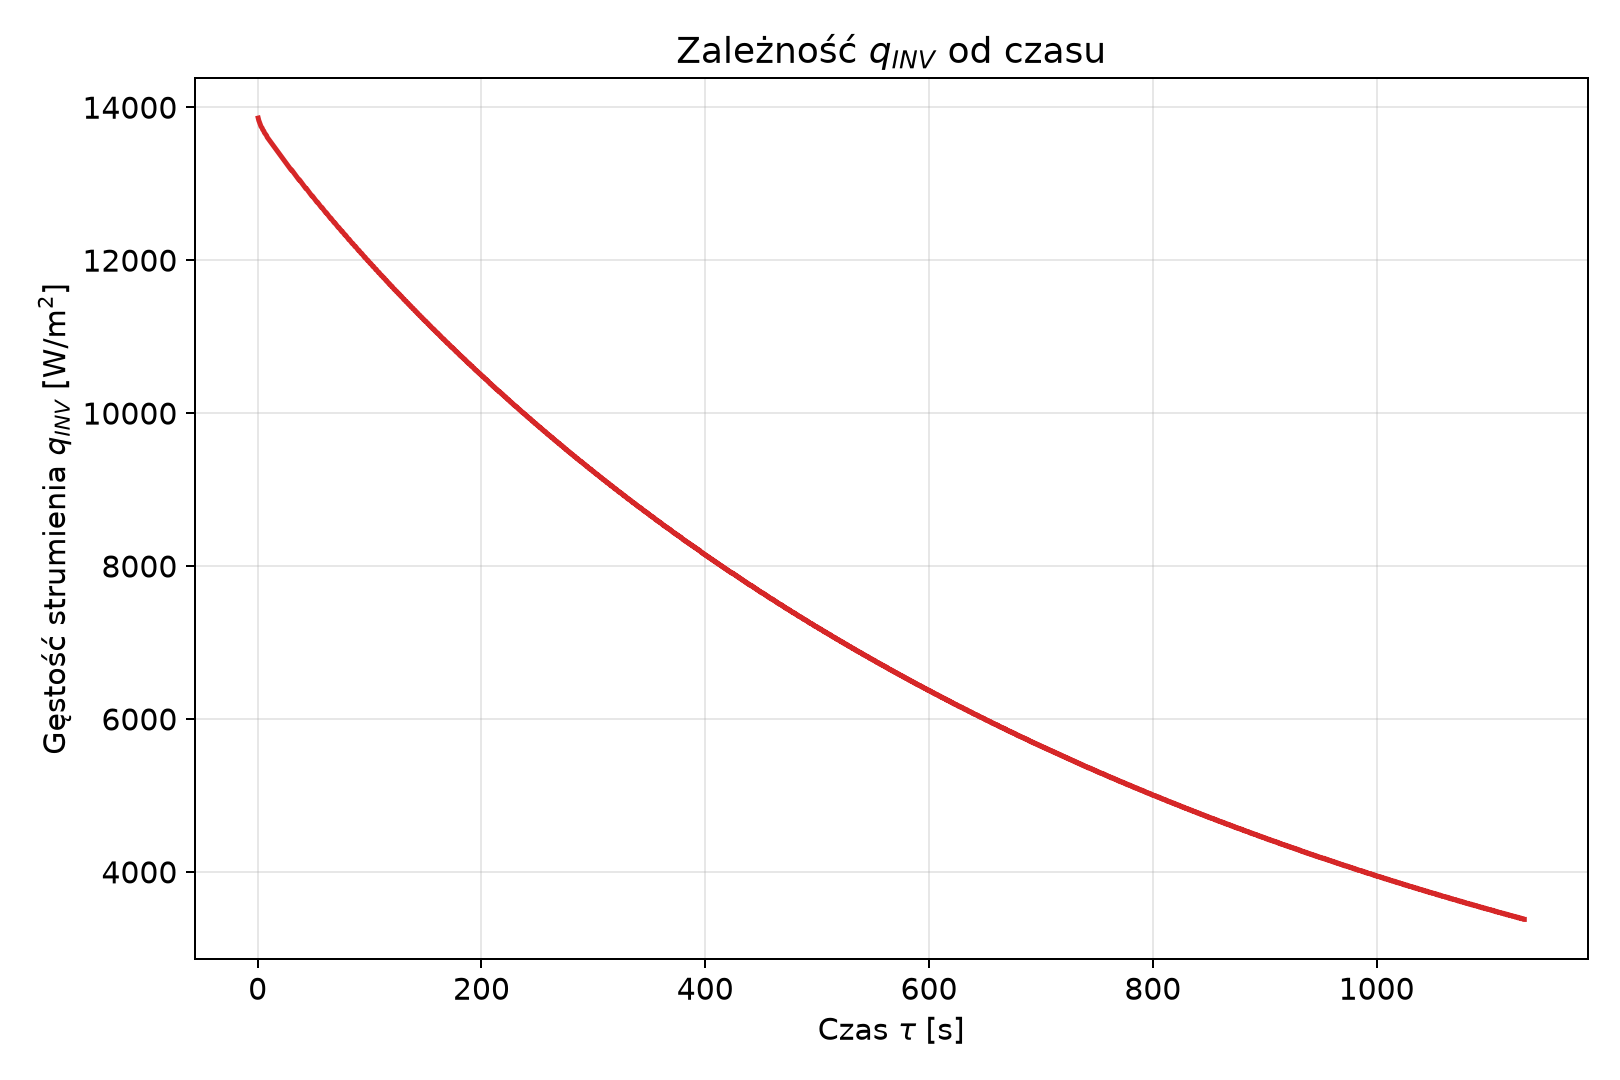
\includegraphics[width=0.92\textwidth]{wykres_qinv_czas.png}
    \caption{Zmiana gęstości strumienia ciepła $q_{\text{inv}}$ w funkcji czasu $\tau$.}
    \label{fig:qinv_czas}
\end{figure}

Z analizowanej tabeli wynika, że gęstość strumienia w pierwszym odczycie wynosiła $13{,}86\text{ kW/m}^2$, a na końcu procesu spadła do $3{,}38\text{ kW/m}^2$. Zależność $q_{\text{inv}}(T_s)$ ma zatem charakter malejący, a ten sam trend obserwuje się w funkcji czasu.

\section{Wnioski}

\begin{enumerate}
    \item Wyznaczona analitycznie wartość całkowitego współczynnika wymiany ciepła dla termometru nr 3 wynosi $\alpha_3 = 32{,}50 \text{ W/(m}^2 \cdot \text{K)}$, a całkowita gęstość strumienia ciepła wynosi $q_3 = 7928{,}07 \text{ W/m}^2$.
    
    \item Głównym mechanizmem przekazywania ciepła w piecu przy analizowanej temperaturze jest promieniowanie --- udziałowi strumienia radiacyjnego $q_{\text{rad}} \approx 6241{,}42 \text{ W/m}^2$ odpowiada aż $\approx 78{,}7\%$ całkowitego strumienia ciepła przekazywanego do próbki.
    
    \item Wszystkie trzy przebiegi obliczeniowe dla $\alpha = 32{,}50 \text{ W/(m}^2 \cdot \text{K)}$ mają charakter monotoniczny i odpowiadają nagrzewaniu próbki od temperatury początkowej do temperatury zbliżonej do temperatury otoczenia pieca. Pełna ocena zgodności z pomiarami wymaga dołączenia szeregu czasowego \texttt{tpomiar.dat}.
    
    \item Wykresy zależności $q_{\text{inv}}(T_s)$ oraz $q_{\text{inv}}(\tau)$ potwierdzają, że gęstość strumienia ciepła wnikającego do wsadu maleje wraz ze wzrostem temperatury powierzchni $T_s$ oraz upływem czasu nagrzewania $\tau$, co wynika ze zmniejszającej się różnicy temperatur między ścianką komory pieca a powierzchnią wsadu.
    
    \item Wyznaczony współczynnik $\alpha_3$ stanowi poprawnie zdefiniowany warunek brzegowy III rodzaju niezbędny do dalszych obliczeń numerycznych i rozwiązywania odwrotnego zagadnienia przewodzenia ciepła.
\end{enumerate}

\end{document}